\documentclass[12pt]{article}

\usepackage{graphicx}
\usepackage{paralist}
\usepackage{listings}
\usepackage{booktabs}
\usepackage{adjustbox}
\usepackage[font=small,labelfont=bf]{caption} 
\usepackage{float}
\restylefloat{table}

\oddsidemargin 0mm
\evensidemargin 0mm
\textwidth 160mm
\textheight 200mm

\pagestyle{plain}
\pagenumbering{arabic}

\newcounter{stepnum}

\title{SE2XB3 Requirements Specification: OptimizeU}
\author{SE2XB3 Group 8, L03}
\date{\today}

\begin{document}

\maketitle
\tableofcontents

\newpage
\section{Introduction}
The purpose of this document is to provide a requirements specification for
building an optimization system for Uber drivers to increase maximum uptime
for drivers and passengers alike.
\section{Domain}
\subsection{Application}
OptimizeU will have the following information:
\begin{itemize}
	\item \textbf{Uber pickups Dataset}:\\
	       Used to generate cluster information and pickup hotspots for
	       drivers to locate and pickup passengers
	\item \textbf{Client-Server Interface}:\\
	       Information is stored server-side. Users (drivers) fetch data
	       from the server by input from the client.
\end{itemize} 
A more detailed functional and non-functional specification will be 
discussed later below.
\subsection{Stakeholders}
The stakeholders and their main relationships are listed below:
\begin{itemize}
	\item \textbf{Drivers}:\\
		These are the primary users of the application; They interact 
		directly with the program by obtaining location hotspots from
		certain times of days to get optimal travel routes and cluster
		visitations. 
	\item \textbf{Passengers}:\\
		Although passengers do not directly access the program, they
		are also considered a major stakeholder due to their relationship
		with drivers; passengers are the customers for the services that
		drivers provide.
\end{itemize}
\subsection{Goals, Expectations and Effects}
\begin{itemize}
	\item \textbf{Maximize driver's uptime and profits}:\\
		By smart optimization of driver's recommended locations and times
		to visit, more time will be spent on fetching passengers instead
		of finding for potential customers.
	\item \textbf{Improve passenger's wait times and safety}:\\
		Since more drivers are directed to passenger hotspots by usage
		of OptimizeU, passengers can enjoy minimized wait times and also
		street crime can be indirectly reduced as passengers spend less time
		waiting outside on streets.
\end{itemize}

\section{Functional Requirements}
The functional requirements will be documented using a use-case document (in
the form of a table), and a use-case diagram.

\begin{table}[H]
 \centering
  \begin{adjustbox}{max width=\textwidth}
  \begin{tabular}{*{2}{|l}|}
  \hline
  \textbf{Name:} & Get Optimized Routes\\
  \hline
  \textbf{Created By:} & SE2XB3 2018 Group 8\\
  \hline
  \textbf{Description:} & Uber driver submits a request for optimized routes to OptimizeU Server\\
  \hline
  \textbf{Actors:} & Uber driver, OptimizeU Server, OptimizeU Client User Interface\\
  \hline
  \textbf{Preconditions:} & 1. Uber driver has access to the Client User Interface\\
  						  & 2. OptimizeU has fully functional Client and Server\\
  						  & 3. Driver is in New York City area\\
  						  &	4. Dataset and server security is not compromised\\
  \hline
  \textbf{Postconditions:} & 1. Client retrieves and displays requested information successfully\\
                          & 2. Drivers get optimized routes from OptimizeU\\
  \hline
  \textbf{Flow:} & 1. Driver makes a request to OptimizeU server through the client\\
                 & 2. OptimizeU sends information about driver's location and timeframe to server\\
                 & 3. Server fetches dataset\\
                 & 4. Server uses dataset and driver information to process an optimized output\\
                 & 5. Server sends output information back to client\\
                 & 6. Driver uses information received as their driving route\\
  \hline
  \textbf{Alternate Flow:} & In Step 2, if driver's time is abnormal (e.g. past midnight times)\\
                           & 1. Proceed as normal up to step 5\\
                           & 2. Send a warning about possibly inaccurate information together with the \\
                           &    output data back to the client\\
                           & 3. Display warning to driver\\
  \hline
\end{tabular}
\end{adjustbox}
  \caption{Use Case Document in Table form}
  \label{usecase}
\end{table}
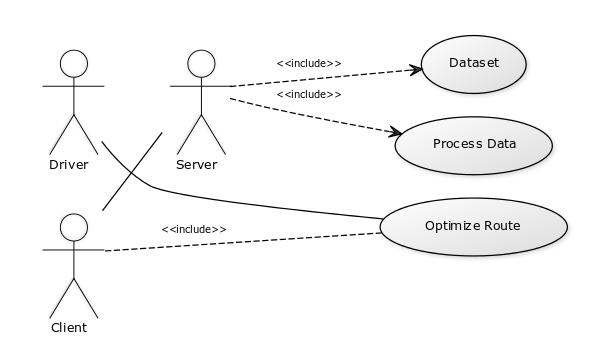
\includegraphics[width=100mm,scale=0.9]{Uses.png}
\captionof{figure}{Uses Case Diagram}


\section{Non-Functional Requirements}
\subsection{Performance and Accuracy of Results}
OptimizeU should have the following capabilities:
\begin{itemize}
	\item \textbf{Adequate server-client response time:}\\
		Users should expect to get results within a reasonable time frame after submitting
		a request to the OptimizeU server. Depending on server load and external factors,
		users should expect a response within 10 to 15 seconds.
	\item \textbf{Consistent, accurate output}\\
		OptimizeU should consistently generate meaningful output for drivers to act on.
		An example being clustering that makes sense (e.g. a mega-cluster covering an 
		entire city wouldn't be of any use); or paths that are always minimal.
\end{itemize}
\subsection{Software Quality Attributes}
OptimizeU should possess the following software quality attributes:
\begin{itemize}
	\item \textbf{Reliability:}\\
		Generate optimized paths that are actually of use to the user. See the above
		section on consistency for an example.
	\item \textbf{Security:}\\
		Since this is a client-server interface, users should be assured that 
		any sensitive information sent (for example, location) is properly handled
		and safeguarded against malicious intent. This can probably be done via
		HTTPS. The server should also be protected against attacks, but this will
		not be the main focus of the project.
	\item \textbf{Safety:}\\
		OptimizeU should ensure driver safety by providing appropriate route information.
		For example, routes should obey flow-of-traffic rules. This will probably
		be implemented as an extra feature, as this is not in scope of the project.
	\item \textbf{Portability Issues:}\\
		OptimizeU is portable client-side as it is implemented using HTML. However,
		programmers may have to account for server-side context, but it should not
		be an issue since it is implemented using portable Java code.
\end{itemize}
\section{Requirements on the Development and Maintenance Process}
\subsection{System test procedures}
The following system test must be carried out before the final product is ready:
\begin{itemize}
	\item \textbf{Algorithm testing}\\
		Test critical algorithms rigorously to ensure that accurate information
		is always delivered to users.
	\item \textbf{Server testing}\\
		Test that the server functions as intended to process client input and
		sends correct information.
	\item \textbf{Client interface testing}\\
		Ensure that client interface are standardized to HTML and provide
		an acceptable user experience.
\end{itemize}
\subsection{Priorities of Required Functions}
A list of required functions (on server backend) and their corresponding priorities are listed:
\begin{itemize}
	\item \textbf{k-medoids}\\
		The clustering algorithm that is planned to be implemented. Must work on
		every occasion save on faulty or abnormal user input
	\item \textbf{Kruskal}\\
		The minimum-spanning tree path generation. Dependent on the correctness
		of k-medoids, but must also properly generate a MST on every clusters.
\end{itemize}
\subsection{Likely changes to System Maintenance Procedures}
\begin{itemize}
	\item Seperate tests may be carried out on similar algorithms (e.g. Prim vs Kruskal,
	k-means vs k-medoids etc.) if performance suffers. Change if necessary as well.
	\item Client-side maintenance as an iterative process: Since user experience 
	relies on feedback to a certain extent, the client-side interface may be
	constantly modified, On each iteration, its communication with the server
	must always be tested to ensure flawless communication.
	\item Security testing: Testing to check server compromisation should be carried
	out AND MODIFIED periodically to ensure that attackers do not gain improper access to 
	server-side information or user information. 
\end{itemize}
\end{document}